\documentclass[tikz]{standalone}
\usepackage{amsmath}
\begin{document}
% Kanvas gelap: 1000x560 => skala 1cm ~ 56px; pakai x=100,y=40 unit scaled
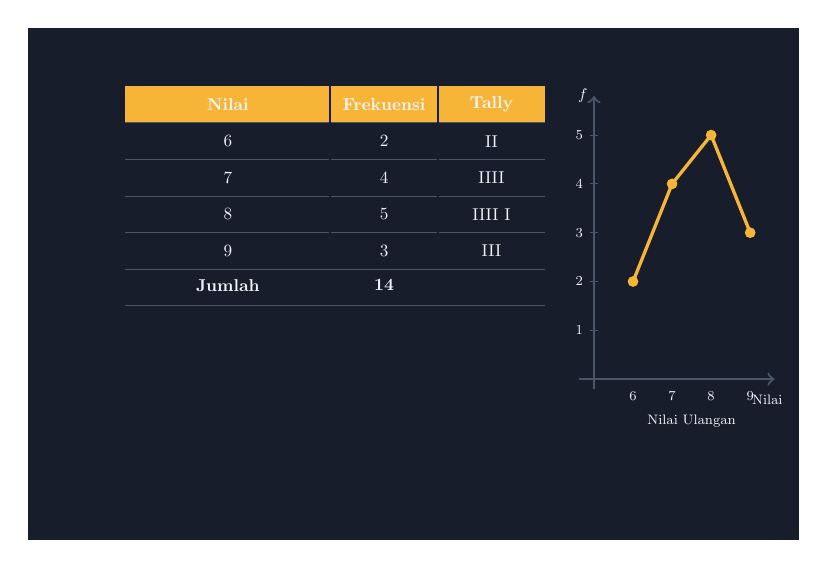
\begin{tikzpicture}[x=1cm,y=1cm, scale=0.62, every node/.style={transform shape}]
\definecolor{bg}{HTML}{171D2B}
\definecolor{ak}{HTML}{F7B538}
\definecolor{line}{HTML}{4A5568}
\definecolor{teks}{HTML}{F1F5F9}
\definecolor{bar}{HTML}{3B82F6}
\fill[bg] (-1,-1.7) rectangle (14.8,8.8);
% --- kiri: tabel frekuensi ---
\def\cl{1.0} % kolom kiri nilai, lebar 4.2
\def\cf{5.2} % kolom frekuensi, lebar 2.2
\def\cc{7.4} % kolom tally, lebar 2.2
\def\top{7.6}
\def\rh{0.75}
% header
\fill[ak] (\cl,\top) rectangle (\cl+4.2,\top-\rh);
\fill[ak] (\cf,\top) rectangle (\cf+2.2,\top-\rh);
\fill[ak] (\cc,\top) rectangle (\cc+2.2,\top-\rh);
\node[teks,font=\bfseries] at (\cl+2.1,\top-\rh/2) {Nilai};
\node[teks,font=\bfseries] at (\cf+1.1,\top-\rh/2) {Frekuensi};
\node[teks,font=\bfseries] at (\cc+1.1,\top-\rh/2) {Tally};
% garis vertikal header
\draw[bg,thick] (\cf,\top) -- (\cf,\top-\rh);
\draw[bg,thick] (\cc,\top) -- (\cc,\top-\rh);
% baris data
\foreach \i/\n/\f/\t in {1/6/2/II, 2/7/4/IIII, 3/8/5/IIII I, 4/9/3/III}{
  \pgfmathsetmacro\y{\top-\rh*\i}
  \draw[line] (\cl,\y) -- (\cc+2.2,\y);
  \draw[bg,thick] (\cf,\y) -- (\cf,\y+\rh);
  \draw[bg,thick] (\cc,\y) -- (\cc,\y+\rh);
  \node[teks] at (\cl+2.1,\y-\rh/2) {\n};
  \node[teks] at (\cf+1.1,\y-\rh/2) {\f};
  \node[teks] at (\cc+1.1,\y-\rh/2) {\t};
}
% garis penutup tabel
\draw[line] (\cl,\top-\rh*5) -- (\cc+2.2,\top-\rh*5);
% total
\node[teks,font=\bfseries] at (\cl+2.1,\top-\rh*5-\rh/2+0.05) {Jumlah};
\node[teks,font=\bfseries] at (\cf+1.1,\top-\rh*5-\rh/2+0.05) {14};
\draw[line] (\cl,\top-\rh*6) -- (\cc+2.2,\top-\rh*6);
% label skor di kolom tally (perhatikan tally IIIII dengan garis silang di 5)
% --- kanan: diagram garis ---
\begin{scope}[shift={(10.6,1.6)}]
  \def\h{5.2}
  \draw[->,line,thick] (-0.3,0) -- (3.7,0);
  \node[teks,below,font=\footnotesize] at (3.55,-0.2) {Nilai};
  \draw[->,line,thick] (0,-0.2) -- (0,\h+0.6) node[teks,left] {\small $f$};
  % skala y 0..5
  \foreach \v in {1,2,3,4,5}{
    \draw[line] (-0.08,\v) -- (0.08,\v);
    \node[teks,left,font=\footnotesize] at (-0.1,\v) {\v};
  }
  % titik data (6,2)(7,4)(8,5)(9,3), jarak x = 0.8
  \draw[ak,very thick] (0.8,2) -- (1.6,4) -- (2.4,5) -- (3.2,3);
  \foreach \x/\y in {0.8/2,1.6/4,2.4/5,3.2/3}{
    \fill[ak] (\x,\y) circle (0.11);
  }
  \node[teks,font=\footnotesize] at (0.8,-0.35) {6};
  \node[teks,font=\footnotesize] at (1.6,-0.35) {7};
  \node[teks,font=\footnotesize] at (2.4,-0.35) {8};
  \node[teks,font=\footnotesize] at (3.2,-0.35) {9};
  \node[teks,font=\footnotesize] at (2.0,-0.85) {Nilai Ulangan};
\end{scope}
\end{tikzpicture}
\end{document}
